\documentclass[border=10pt]{standalone}
%%%<
\usepackage{verbatim}
%%%>
\usepackage{pgfplots}
\pgfplotsset{width=7cm,compat=1.8}
\begin{comment}
:Title: Moebius strip
:Tags: 3D;Surface plots;Mathematics
:Author: Jake
:Slug: moebius-strip

A Moebius strip plot.

This code was written by Jake on TeX.SE.
\end{comment}
\begin{document}
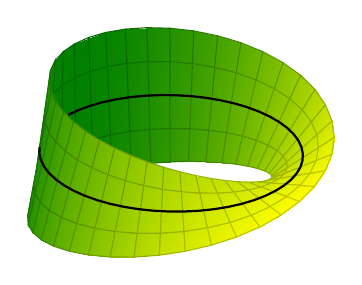
\begin{tikzpicture}
  \begin{axis}[
    hide axis,
    view = {40}{40}
  ]
  \addplot3 [
    surf,
    colormap/greenyellow,
    shader     = faceted interp,
    point meta = x,
    samples    = 40,
    samples y  = 5,
    z buffer   = sort,
    domain     = 0:360,
    y domain   =-0.5:0.5
  ] (
    {(1+0.5*y*cos(x/2)))*cos(x)},
    {(1+0.5*y*cos(x/2)))*sin(x)},
    {0.5*y*sin(x/2)}
  );

  \addplot3 [
    samples=50,
    domain=-145:180, % The domain needs to be adjusted manually,
                     % depending on the camera angle, unfortunately
    samples y=0,
    thick
  ] (
    {cos(x)},
    {sin(x)},
    {0}
  );
  \end{axis}
\end{tikzpicture}
\end{document}